Using the recently release Intel SGX SDK, we implmented TC Server as an SGX
application.  The programming model of SGX applications is to seperate out the
security-sensitive part of an application into a trusted partition, while the
remainder of the application is deemed untrusted.  The trusted partition is
later loaded into a SGX enclave and execuate there. 

The idea behind the programming model is that the major body of the application
is just a normal C/C++ application that is execuated as usual. The trusted part
is invoked by the application when the application needs to perform a
security-sensitive task, such as to generate a key pair only unknown to the
trusted part. To call a function in the enclave, the untrusted part first
prepare the arguments and issue a \texttt{EENTER} instruction with the address
of functions being called as arguments.  After the issueing of \texttt{EENTER},
control is transferred to the program insided the enclave until it returns or a
Exit Event happens~\cite{sgxman}. This process is referred to as making
\emph{ecall}s in the SGX documentation.

An SGX enclave is an isolated execution envirtonment where the enclave program
can be loaded and execuated. As a result of being isolated, the flexibility of
enclave programs is trimmed. For example, some instructions, such as IO
instructions and system calls\fan{add more}, are not allowed in the enclave.
Thus an enclave program has no access to the services and resources provided by
operating systems (such as file systems and networking). In order for the enclave
program to make use of OS services, the enclave program first have to exit the 
enclave. The \texttt{EEXIT} takes a function pointer as input and will transfer
control to that address after exiting. Ususally the function being pointed to
is a wrapper function of a system call, where it first make the system call and
gather the result, then it transfer control back to the enclave code so that the
enclave can make use of the data. This process is referred as making \emph{ocall}
in the SGX documentation.

In the context of TC Server, the trusted part implements Figure. \fan{ref to prog},
which emcompasses a TLS layer, a partical HTTP protocol, a set of algorithms that
can extract information from web pages, and a request handler that
can parse and generate Ethereum transactions. 
The untrusted part of TC Server is the \medname, which roughly emcompasses of
two parts: (1) an access point to various OS services and (2) interfaces with
users and Ethereum blockchain. Figure \ref{fig:tcserver_impl} summarizes these
components and their interaction.

\begin{figure}[h]
    \centering
    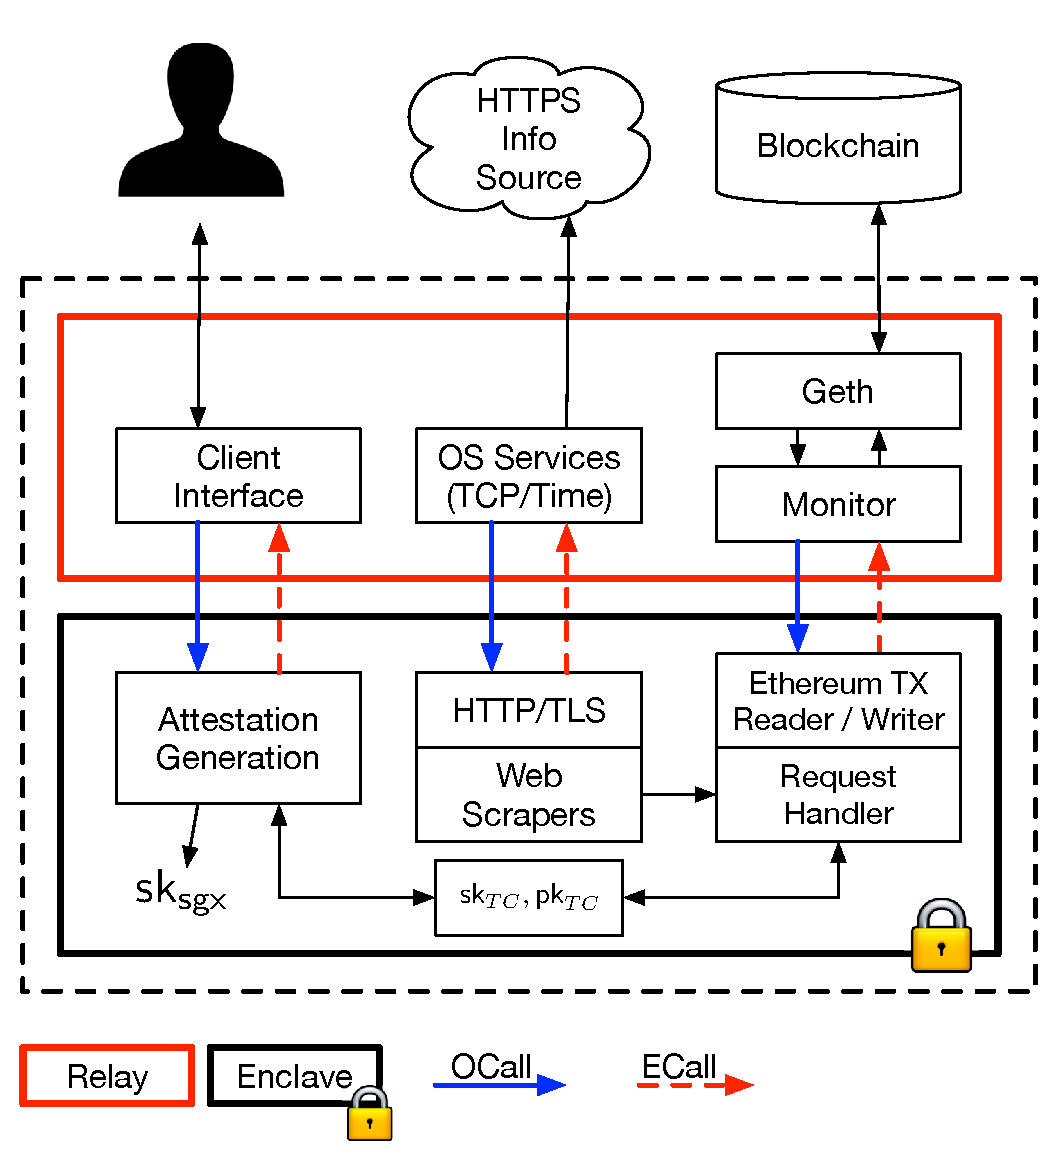
\includegraphics[width=0.4\textwidth]{figures/impl}
    \caption{Detailed Architecture of TC Server}
    \label{fig:tcserver_impl}
\end{figure}

\subsubsection{The \medname}

\paragraph{Attestation Server.} 

\paragraph{OS Services.}

\paragraph{Blockchain Interface.}

\subsubsection{The \encname}

\paragraph{HTTPS in the \encname}
\paragraph{Info Extraction}
\paragraph{Request Handler}
\paragraph{Attestation Generation}
\paragraph{Key Management}
